\section{Text3D Class Reference}
\label{classText3D}\index{Text3D@{Text3D}}
{\tt \#include $<$text3d.h$>$}

Inheritance diagram for Text3D::\begin{figure}[H]
\begin{center}
\leavevmode
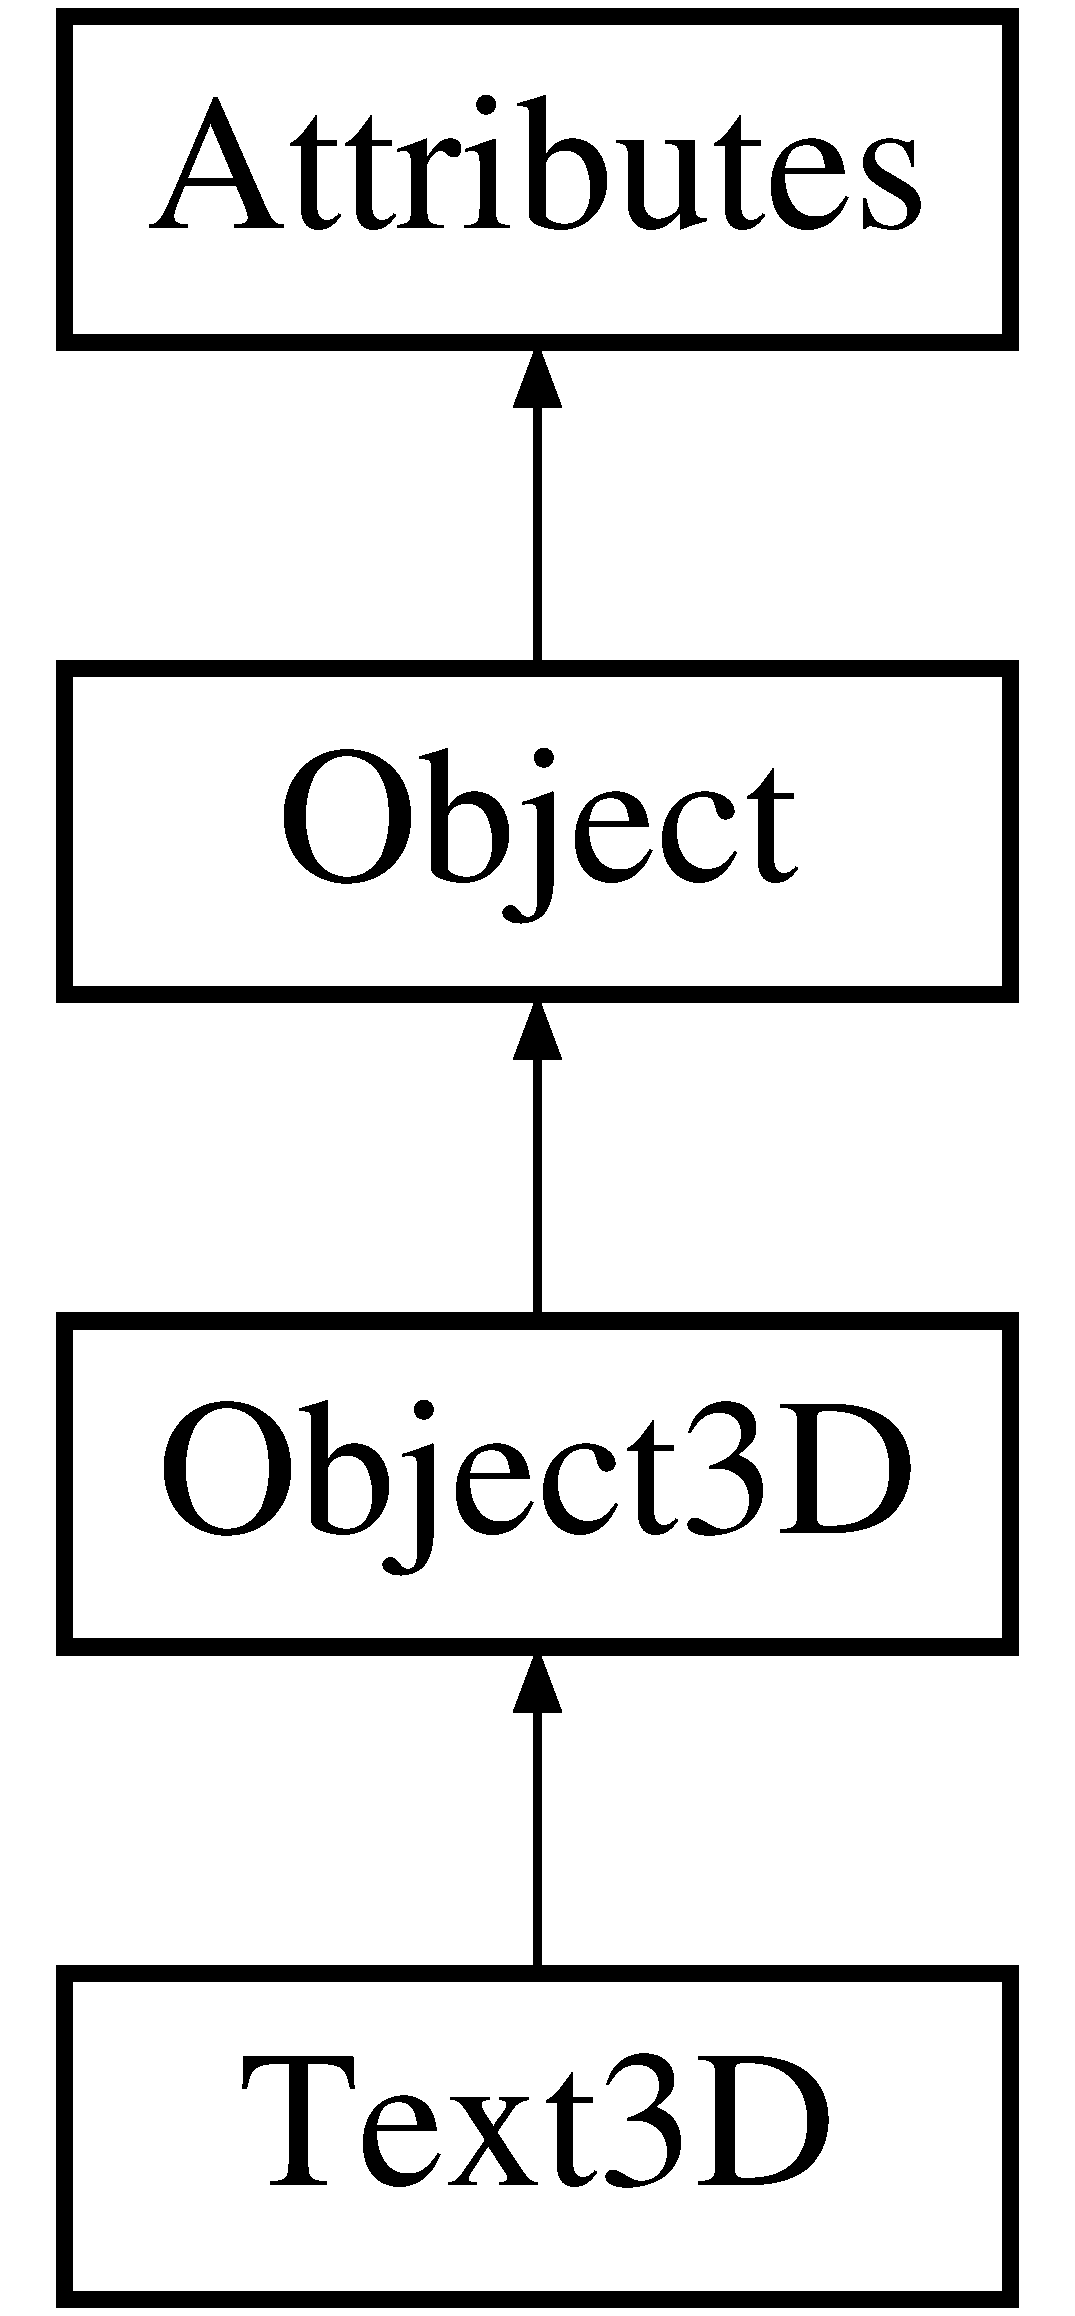
\includegraphics[height=4cm]{classText3D}
\end{center}
\end{figure}
\subsection*{Public Methods}
\begin{CompactItemize}
\item 
{\bf Text3D} ()
\item 
{\bf Text3D} ({\bf Coordinate3D} $\ast${\bf place}, std::string {\bf contents})
\item 
{\bf $\sim$Text3D} ()
\item 
void {\bf set\-Justification} ({\bf Text::Text\-Justifications} {\bf justification})
\item 
{\bf Text::Text\-Justifications} {\bf get\-Justification} ()
\item 
std::pair$<$ double, double $>$ {\bf get\-Depth\-Range} ()
\item 
void {\bf render} ({\bf Figure} $\ast$, double x\-Offset, double y\-Offset, double scale, double distance, double min\-Depth, double max\-Depth, int min\-Fig\-Depth=0, int max\-Fig\-Depth=999)
\item 
void {\bf apply\-Matrix} ({\bf Matrix}$<$ double $>$ $\ast$)
\item 
void {\bf translate} ({\bf Coordinate3D} $\ast$)
\item 
void {\bf write} (std::ostream \&stream) const
\end{CompactItemize}
\subsection*{Protected Attributes}
\begin{CompactItemize}
\item 
{\bf Text::Text\-Justifications} {\bf justification}
\item 
{\bf Coordinate3D} $\ast$ {\bf place}
\item 
std::string {\bf contents}
\end{CompactItemize}


\subsection{Detailed Description}
This class handles text objects. This class is derived from {\bf Object} {\rm (p.\,\pageref{classObject})}. \begin{Desc}
\item[Author: ]\par
Anthony Liekens \end{Desc}




\subsection{Constructor \& Destructor Documentation}
\index{Text3D@{Text3D}!Text3D@{Text3D}}
\index{Text3D@{Text3D}!Text3D@{Text3D}}
\subsubsection{\setlength{\rightskip}{0pt plus 5cm}Text3D::Text3D ()}\label{classText3D_a0}


Constructor. Constructs a text object \index{Text3D@{Text3D}!Text3D@{Text3D}}
\index{Text3D@{Text3D}!Text3D@{Text3D}}
\subsubsection{\setlength{\rightskip}{0pt plus 5cm}Text3D::Text3D ({\bf Coordinate3D} $\ast$ {\em place}, std::string {\em contents})}\label{classText3D_a1}


Constructor. Constructs a text object \begin{Desc}
\item[Parameters: ]\par
\begin{description}
\item[{\em 
place}]- Instance of {\bf Coordinate} {\rm (p.\,\pageref{classCoordinate})}. Coordinates where the text object will be placed. \item[{\em 
contents}]- string \end{description}
\end{Desc}
\index{Text3D@{Text3D}!~Text3D@{$\sim$Text3D}}
\index{~Text3D@{$\sim$Text3D}!Text3D@{Text3D}}
\subsubsection{\setlength{\rightskip}{0pt plus 5cm}Text3D::$\sim$Text3D ()}\label{classText3D_a2}




\subsection{Member Function Documentation}
\index{Text3D@{Text3D}!applyMatrix@{applyMatrix}}
\index{applyMatrix@{applyMatrix}!Text3D@{Text3D}}
\subsubsection{\setlength{\rightskip}{0pt plus 5cm}void Text3D::apply\-Matrix ({\bf Matrix}$<$ double $>$ $\ast$)\hspace{0.3cm}{\tt  [virtual]}}\label{classText3D_a7}




Implements {\bf Object3D} {\rm (p.\,\pageref{classObject3D_a2})}.\index{Text3D@{Text3D}!getDepthRange@{getDepthRange}}
\index{getDepthRange@{getDepthRange}!Text3D@{Text3D}}
\subsubsection{\setlength{\rightskip}{0pt plus 5cm}std::pair$<$ double, double $>$ Text3D::get\-Depth\-Range ()\hspace{0.3cm}{\tt  [virtual]}}\label{classText3D_a5}




Implements {\bf Object3D} {\rm (p.\,\pageref{classObject3D_a0})}.\index{Text3D@{Text3D}!getJustification@{getJustification}}
\index{getJustification@{getJustification}!Text3D@{Text3D}}
\subsubsection{\setlength{\rightskip}{0pt plus 5cm}{\bf Text::Text\-Justifications} Text3D::get\-Justification ()\hspace{0.3cm}{\tt  [inline]}}\label{classText3D_a4}


Returns the text justification \begin{Desc}
\item[Returns: ]\par
Instance of Text\-Justifications \end{Desc}
\index{Text3D@{Text3D}!render@{render}}
\index{render@{render}!Text3D@{Text3D}}
\subsubsection{\setlength{\rightskip}{0pt plus 5cm}void Text3D::render ({\bf Figure} $\ast$, double {\em x\-Offset}, double {\em y\-Offset}, double {\em scale}, double {\em distance}, double {\em min\-Depth}, double {\em max\-Depth}, int {\em min\-Fig\-Depth} = 0, int {\em max\-Fig\-Depth} = 999)\hspace{0.3cm}{\tt  [virtual]}}\label{classText3D_a6}




Implements {\bf Object3D} {\rm (p.\,\pageref{classObject3D_a1})}.\index{Text3D@{Text3D}!setJustification@{setJustification}}
\index{setJustification@{setJustification}!Text3D@{Text3D}}
\subsubsection{\setlength{\rightskip}{0pt plus 5cm}void Text3D::set\-Justification ({\bf Text::Text\-Justifications} {\em justification})\hspace{0.3cm}{\tt  [inline]}}\label{classText3D_a3}


Set the text justification \begin{Desc}
\item[Parameters: ]\par
\begin{description}
\item[{\em 
justification}]Text\-Justifications \end{description}
\end{Desc}
\begin{Desc}
\item[Returns: ]\par
void \end{Desc}
\index{Text3D@{Text3D}!translate@{translate}}
\index{translate@{translate}!Text3D@{Text3D}}
\subsubsection{\setlength{\rightskip}{0pt plus 5cm}void Text3D::translate ({\bf Coordinate3D} $\ast$)\hspace{0.3cm}{\tt  [virtual]}}\label{classText3D_a8}




Implements {\bf Object3D} {\rm (p.\,\pageref{classObject3D_a3})}.\index{Text3D@{Text3D}!write@{write}}
\index{write@{write}!Text3D@{Text3D}}
\subsubsection{\setlength{\rightskip}{0pt plus 5cm}void Text3D::write (std::ostream \& {\em stream}) const\hspace{0.3cm}{\tt  [virtual]}}\label{classText3D_a9}


Write the text object to a given outstream. \begin{Desc}
\item[Parameters: ]\par
\begin{description}
\item[{\em 
stream}]output stream \end{description}
\end{Desc}
\begin{Desc}
\item[Returns: ]\par
void \end{Desc}


Reimplemented from {\bf Object} {\rm (p.\,\pageref{classObject_a3})}.

\subsection{Member Data Documentation}
\index{Text3D@{Text3D}!contents@{contents}}
\index{contents@{contents}!Text3D@{Text3D}}
\subsubsection{\setlength{\rightskip}{0pt plus 5cm}std::string Text3D::contents\hspace{0.3cm}{\tt  [protected]}}\label{classText3D_n2}


\index{Text3D@{Text3D}!justification@{justification}}
\index{justification@{justification}!Text3D@{Text3D}}
\subsubsection{\setlength{\rightskip}{0pt plus 5cm}{\bf Text::Text\-Justifications} Text3D::justification\hspace{0.3cm}{\tt  [protected]}}\label{classText3D_n0}


\index{Text3D@{Text3D}!place@{place}}
\index{place@{place}!Text3D@{Text3D}}
\subsubsection{\setlength{\rightskip}{0pt plus 5cm}{\bf Coordinate3D}$\ast$ Text3D::place\hspace{0.3cm}{\tt  [protected]}}\label{classText3D_n1}




The documentation for this class was generated from the following files:\begin{CompactItemize}
\item 
{\bf text3d.h}\item 
{\bf text3d.cpp}\end{CompactItemize}
